\documentclass[12pt]{article}

\usepackage{amsmath}
\usepackage{latexsym}
\usepackage{amstext}
\usepackage{array}
\usepackage{multirow}
\usepackage{graphicx}
\usepackage{caption}
\usepackage{subcaption}


%\usepackage{subcaption}

\pagestyle{plain}


\begin{document}
\title{Random loops -Supplementary material}

\begin{figure}[H]
 \begin{subfigure}[b]{0.3\textwidth}
 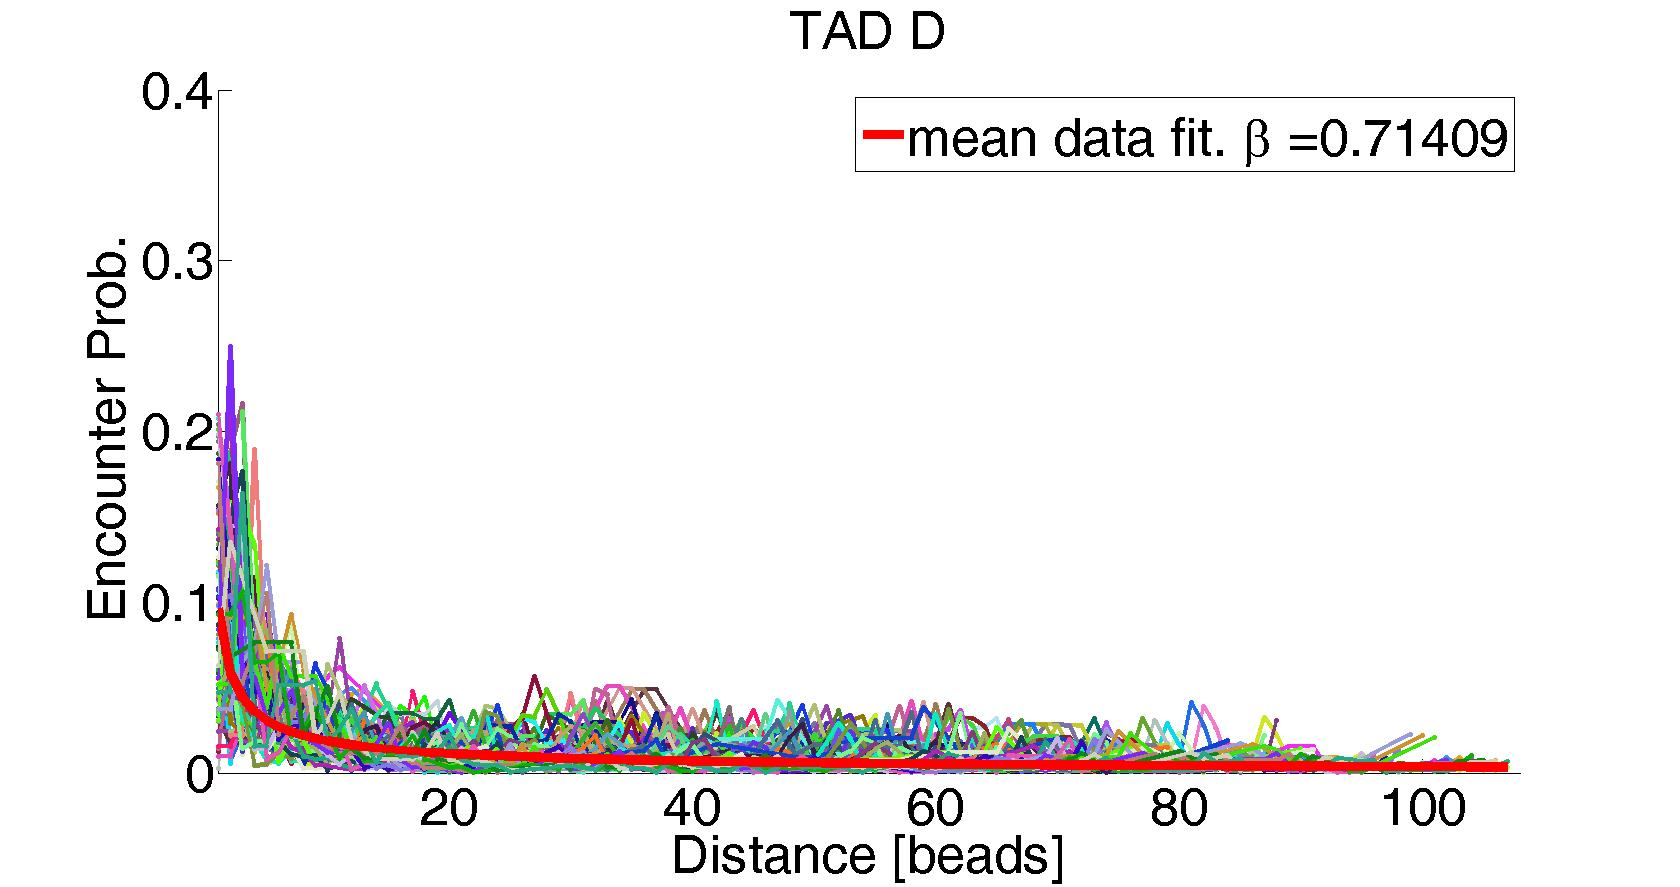
\includegraphics[scale=0.2]{meanDataFitTADD}
 \caption{}
 \end{subfigure}
 
 \begin{subfigure}[b]{0.3\textwidth}
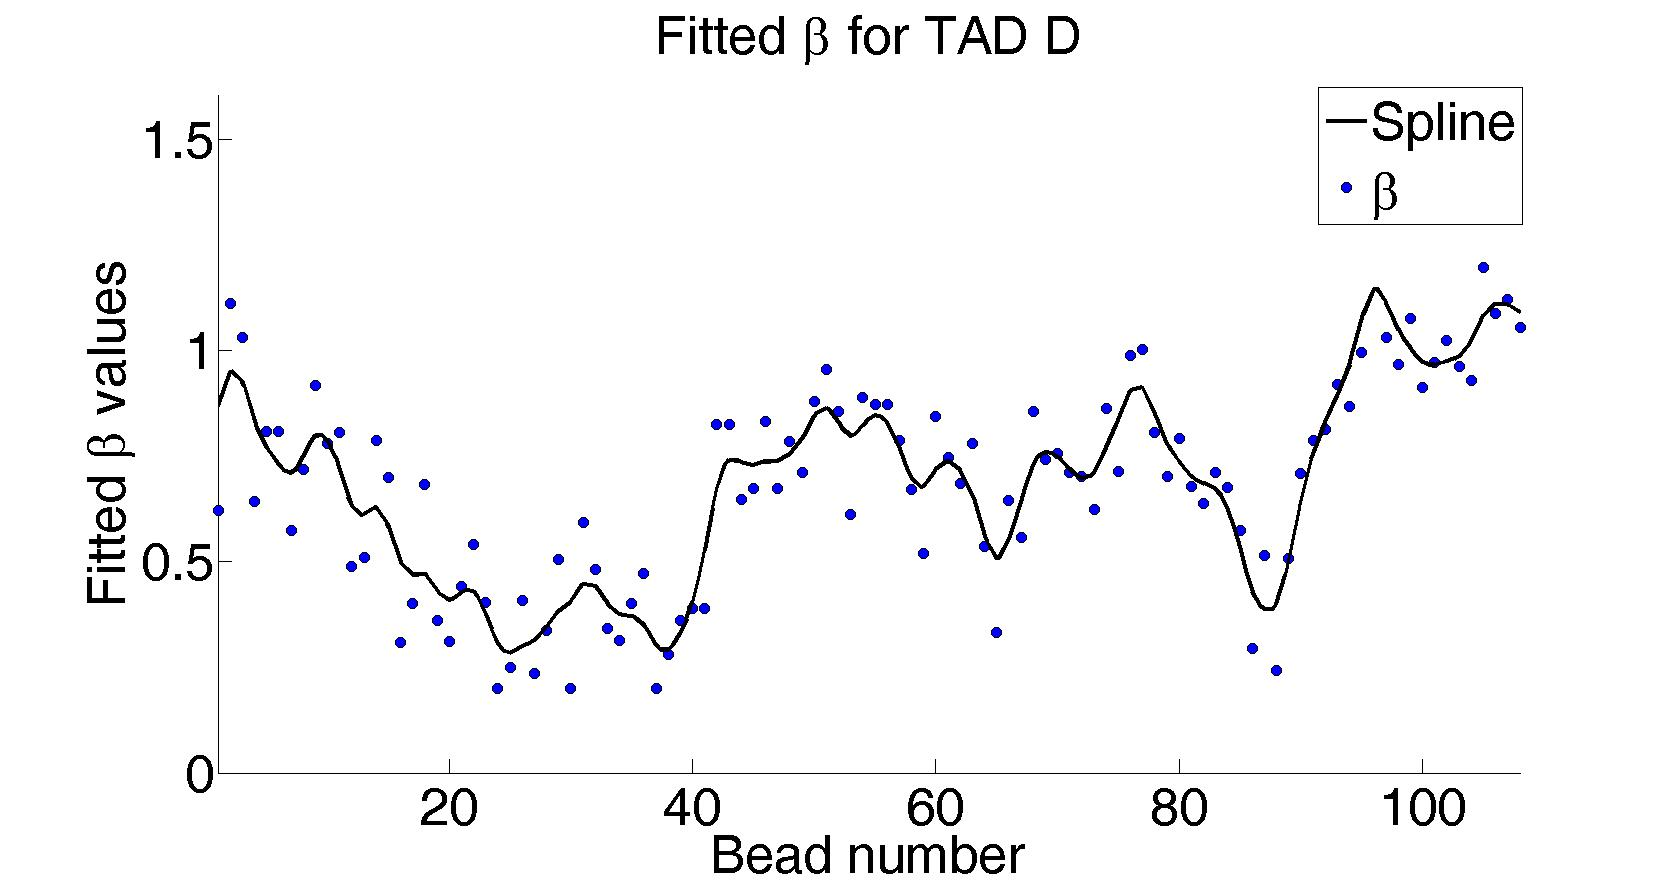
\includegraphics[scale=0.2]{fittedExpValuesWithSplineAverageTADD}
\caption{}
 \end{subfigure}
\caption{The encounter probability and the fitted $\beta$ values for TAD D.}
\end{figure}

\begin{figure}[H]
 \begin{subfigure}[b]{0.3\textwidth}
 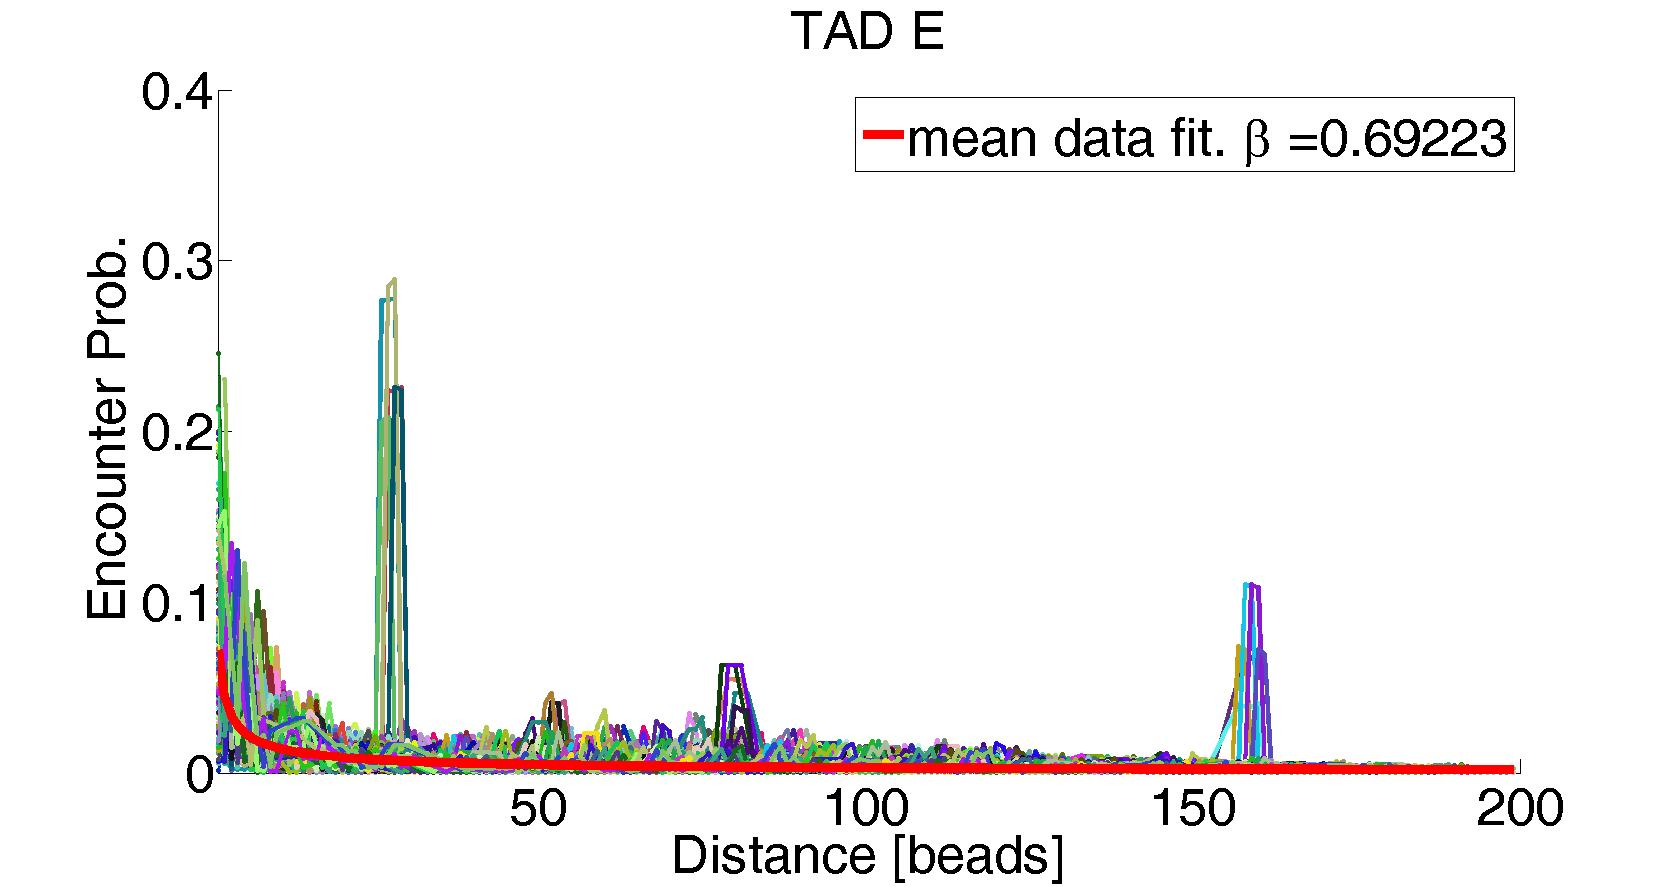
\includegraphics[scale=0.2]{meanDataFitTADE}
 \caption{}
 \end{subfigure}
 
 \begin{subfigure}[b]{0.3\textwidth}
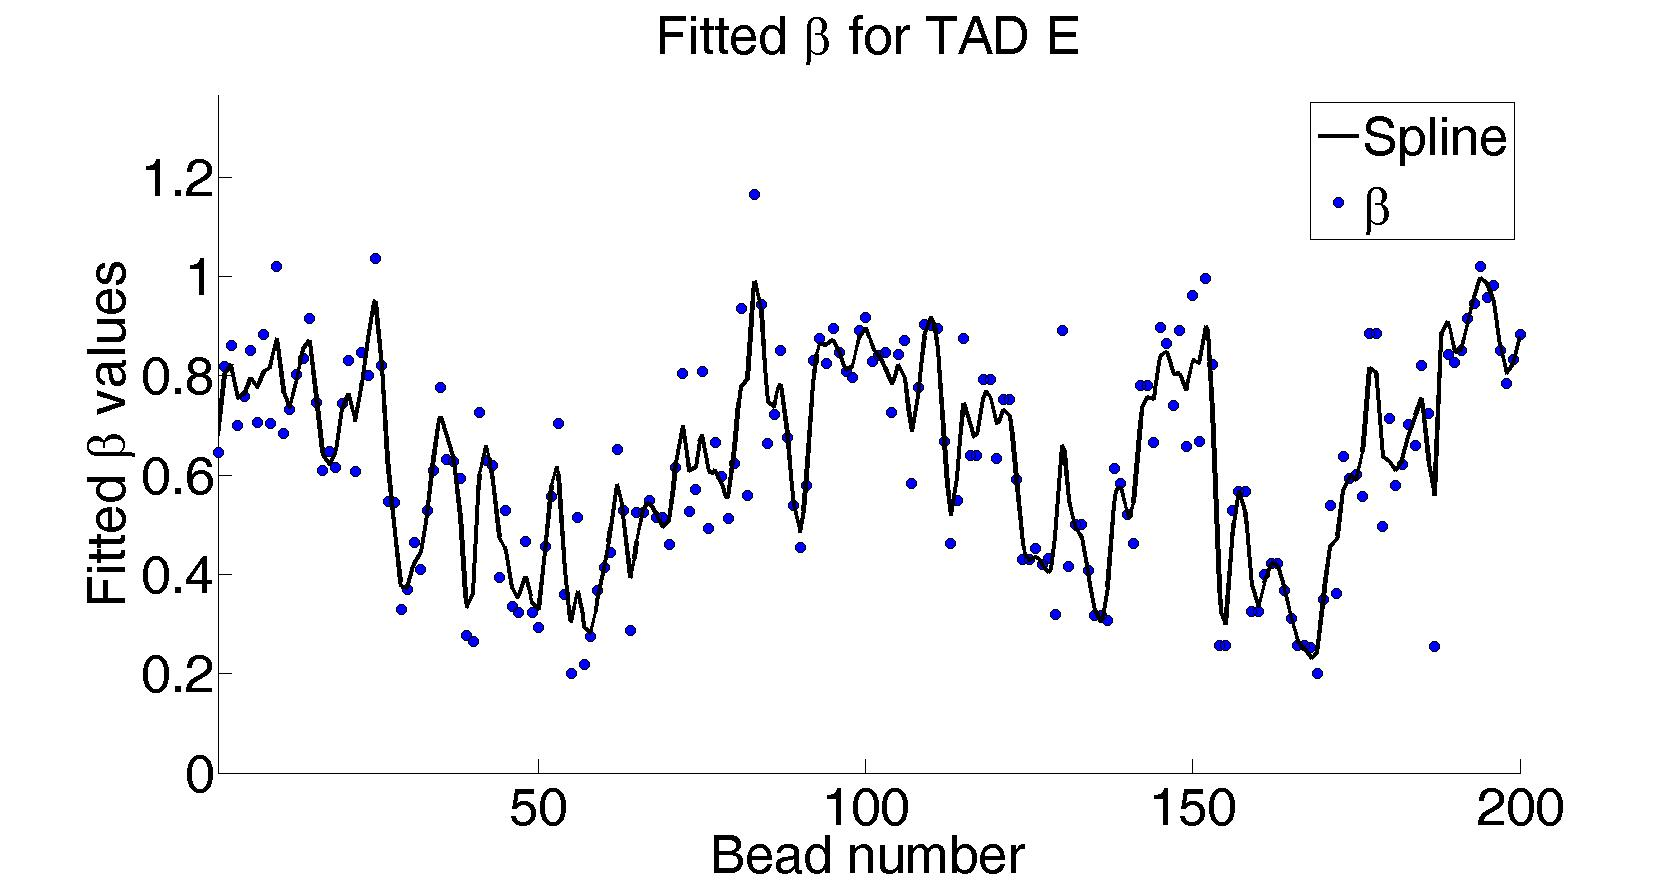
\includegraphics[scale=0.2]{fittedExpValuesWithSplineAverageTADE}
\caption{}
 \end{subfigure}
\caption{The encounter probability and the fitted $\beta$ values for TAD E.}
\end{figure}
\subsection{Peak Calling}

To accurately identify pair of beads that interact more frequently than expected, we ran a peak calling procedure on the 5C probability data of each TAD separately and for the region between TADs. We smooth the encounter frequency signal, taken from all genomic distances, using loess smoothing technique to represent the expected background encounter signal,$E(d)$, and calculate its standard deviation $\sigma_E$. The background Z-score distribution is calculated using all data by $z_B=\frac{O_{i(d)}(d)-E(d)}{\sigma_E}$, for each $i(d)=1,..,N(d)$, with $N(d)$ the number of observations available for genomic distance $d$. A Weibull distribution is fitted to the background signal, where negative values $Z_B$ are treated as censored observations. We then estimate the threshold value, $T_B$, above which z-scores are considered as global outliers of the data, as the 0.99 percent of this distribution. The value of $T_B$ will be used in judging observations in particular genomic distances for being peaks.

For each genomic distance $d$, we calculate a z-score for all available observations at that distance by $z({\{i\}_d})=\frac{O({\{i\}_d})-E(d)}{\sigma_{O}(d)}$ and fit a Weibull distribution to it, truncating negative values. The Weibuul CDF is used to calculate a rejection value $T_d$ above which observation at genomic distance $d$ are considered peaks. 

We estimate a new global rejection value based on the distribution of rejection values obtained for $d$ and the back ground, by calculating the $T = \frac{T_d-T_B}{\sigma_T}$ and fitting it with a Weibull distribution. We then threshold the data with $T_{global}$ as the 0.99 percent of the $T$  distribution. 

For each peak we find after thresholding, we examine the peak strength in its neighborhood of 5, 10, and 15 genomoic distances. The peak it considered true peak if it is a peak in 2 out of 3 neighborhoods. 
 
\end{document}